%texexptitled======================================================================
% lab1-gcd
%-----------------------------------------------------------------------
%

\documentclass[11pt]{article}

% Package includes

\usepackage{graphicx}
\usepackage{color}
\usepackage{comment}
\usepackage{multirow}
\usepackage{askmaps}
\usepackage{amssymb}
\usepackage{amsmath}
\usepackage{tikz}
\usepackage{circuitikzgit}
\usetikzlibrary{arrows, positioning, shapes.geometric, circuits.logic.US}
\tikzstyle{line}=[draw]
\tikzstyle{arrow}=[draw, -latex]

% Wrap long URLs with hyphens
\PassOptionsToPackage{hyphens}{url}\usepackage{hyperref}
\usepackage{pdftexcmds}
\usepackage{upquote}
\usepackage{textcomp}
\usepackage{minted}
\usepackage[listings]{tcolorbox}
\usepackage{enumerate}
\usepackage{enumitem}
\usepackage{mathtools}
\DeclarePairedDelimiter{\ceil}{\Big\lceil}{\Big\rceil}

\tcbset{
texexp/.style={colframe=black, colback=lightgray!15,
         coltitle=white,
         fonttitle=\small\sffamily\bfseries, fontupper=\small, fontlower=\small},
     example/.style 2 args={texexp,
title={Question \thetcbcounter: #1},label={#2}},
}

\newtcolorbox{texexp}[1]{texexp}
\newtcolorbox[auto counter]{texexptitled}[3][]{%
example={#2}{#3},#1}

\setlength{\topmargin}{-0.5in}
\setlength{\textheight}{9in}
\setlength{\oddsidemargin}{0in}
\setlength{\evensidemargin}{0in}
\setlength{\textwidth}{6.5in}

% Useful macros

\newcommand{\note}[1]{{\bf [ NOTE: #1 ]}}
\newcommand{\fixme}[1]{{\bf [ FIXME: #1 ]}}
\newcommand{\wunits}[2]{\mbox{#1\,#2}}
\newcommand{\um}{\mbox{$\mu$m}}
\newcommand{\xum}[1]{\wunits{#1}{\um}}
\newcommand{\by}[2]{\mbox{#1$\times$#2}}
\newcommand{\byby}[3]{\mbox{#1$\times$#2$\times$#3}}


\newenvironment{tightlist}
{\begin{itemize}
 \setlength{\parsep}{0pt}
 \setlength{\itemsep}{-2pt}}
{\end{itemize}}

\newenvironment{titledtightlist}[1]
{\noindent
 ~~\textbf{#1}
 \begin{itemize}
 \setlength{\parsep}{0pt}
 \setlength{\itemsep}{-2pt}}
{\end{itemize}}

% Change spacing before and after section headers

\makeatletter
\renewcommand{\section}
{\@startsection {section}{1}{0pt}
 {-2ex}
 {1ex}
 {\bfseries\Large}}
\makeatother

\makeatletter
\renewcommand{\subsection}
{\@startsection {subsection}{1}{0pt}
 {-1ex}
 {0.5ex}
 {\bfseries\normalsize}}
\makeatother

% Reduce likelihood of a single line at the top/bottom of page

\clubpenalty=2000
\widowpenalty=2000

% Other commands and parameters

\pagestyle{myheadings}
\setlength{\parindent}{0in}
\setlength{\parskip}{10pt}

% Commands for register format figures.

\newcommand{\instbit}[1]{\mbox{\scriptsize #1}}
\newcommand{\instbitrange}[2]{\instbit{#1} \hfill \instbit{#2}}

\newif\ifsolution

\if\issolution1
\newenvironment{solution}
    {\color{red}}
    {\color{black}}
\solutiontrue
\else
\excludecomment{solution}
\solutionfalse
\fi


\graphicspath{{./figs/}}


%-----------------------------------------------------------------------
% Document
%-----------------------------------------------------------------------

\begin{document}
\def\PYZsq{\textquotesingle}


\newcommand{\headertext}{EE142 Problem Set 6}

\title{\vspace{-0.4in}\Large \bf \headertext \vspace{-0.1in}}
\author{Vighnesh Iyer}

\date{\today}
\maketitle

\markboth{\headertext}{\headertext}
\thispagestyle{empty}

\section{Design of a 5-Ghz Linear Microwave Amplifier}

{\color{blue}Use the 32nm PTM HP NMOS model with:

\begin{center}
\begin{tabular}{| l | l |} \hline
    $V_D$ & 0.9 V \\ \hline
    $V_G$ & 0.6 V \\ \hline
    $L$ & 32 nm \\ \hline
    $W_{tot}$ & 20 $\mu$m \\ \hline
    $N_{fingers}$ & 5 \\ \hline
\end{tabular}
\end{center}
}

\begin{figure}[H]
    \centering 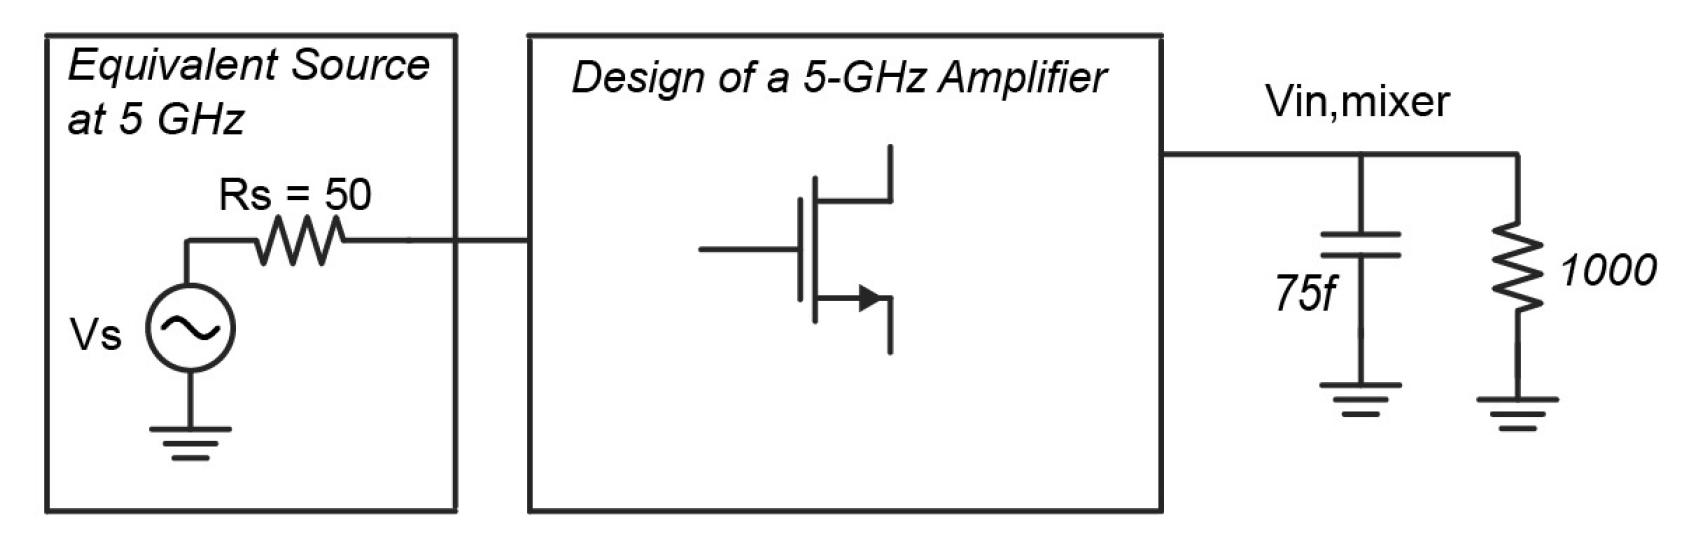
\includegraphics[width=\textwidth-6cm]{system_schematic.png}
\end{figure}

\subsection{Mixer Input Impedance}
{\color{blue}The mixer input is not $50 \Omega$. What will be the problem if this mixer is used as a connector module like the ones sold by MiniCircuits?}

The connector modules assume operation in a $50 \Omega$ environment.
Since the mixer input is $1000 \Omega$, any modules driving it will not be able to achieve the maximum possible power transfer to the mixer. Also, the reflections produced will distort the input waveform to the mixer.

\subsection{Stability Factor}
{\color{blue}Plot the stability factor ($k$), of this device versus frequency.
Is the device unconditionally stable at 1 Ghz?
If not, find a (passive) device load impedance such that the real part of the device
input impedance is negative at 1 Ghz.}

The stability factor ($k$) provides a necessary condition for unconditional stability of a 2-port network. It enforces that the input admittance/impedance of the two-port doesn't have a negative real part.

\begin{align*}
    Y_{in} &= y_{11} - \frac{y_{12}y_{21}}{y_{22} + Y_L} \\
    Y_{out} &= y_{22} - \frac{y_{12}y_{21}}{y_{11} + Y_S} \\
    \text{For instability: } \Re({Y_{in}}) < 0 &\text{ and } \Re(Y_{out}) < 0
\end{align*}

We set up a S-parameter simulation in ADS to calculate the stability factor versus frequency, using the provided transistor sizing and biasing.

\begin{figure}[H]
    \minipage{0.50\textwidth}
    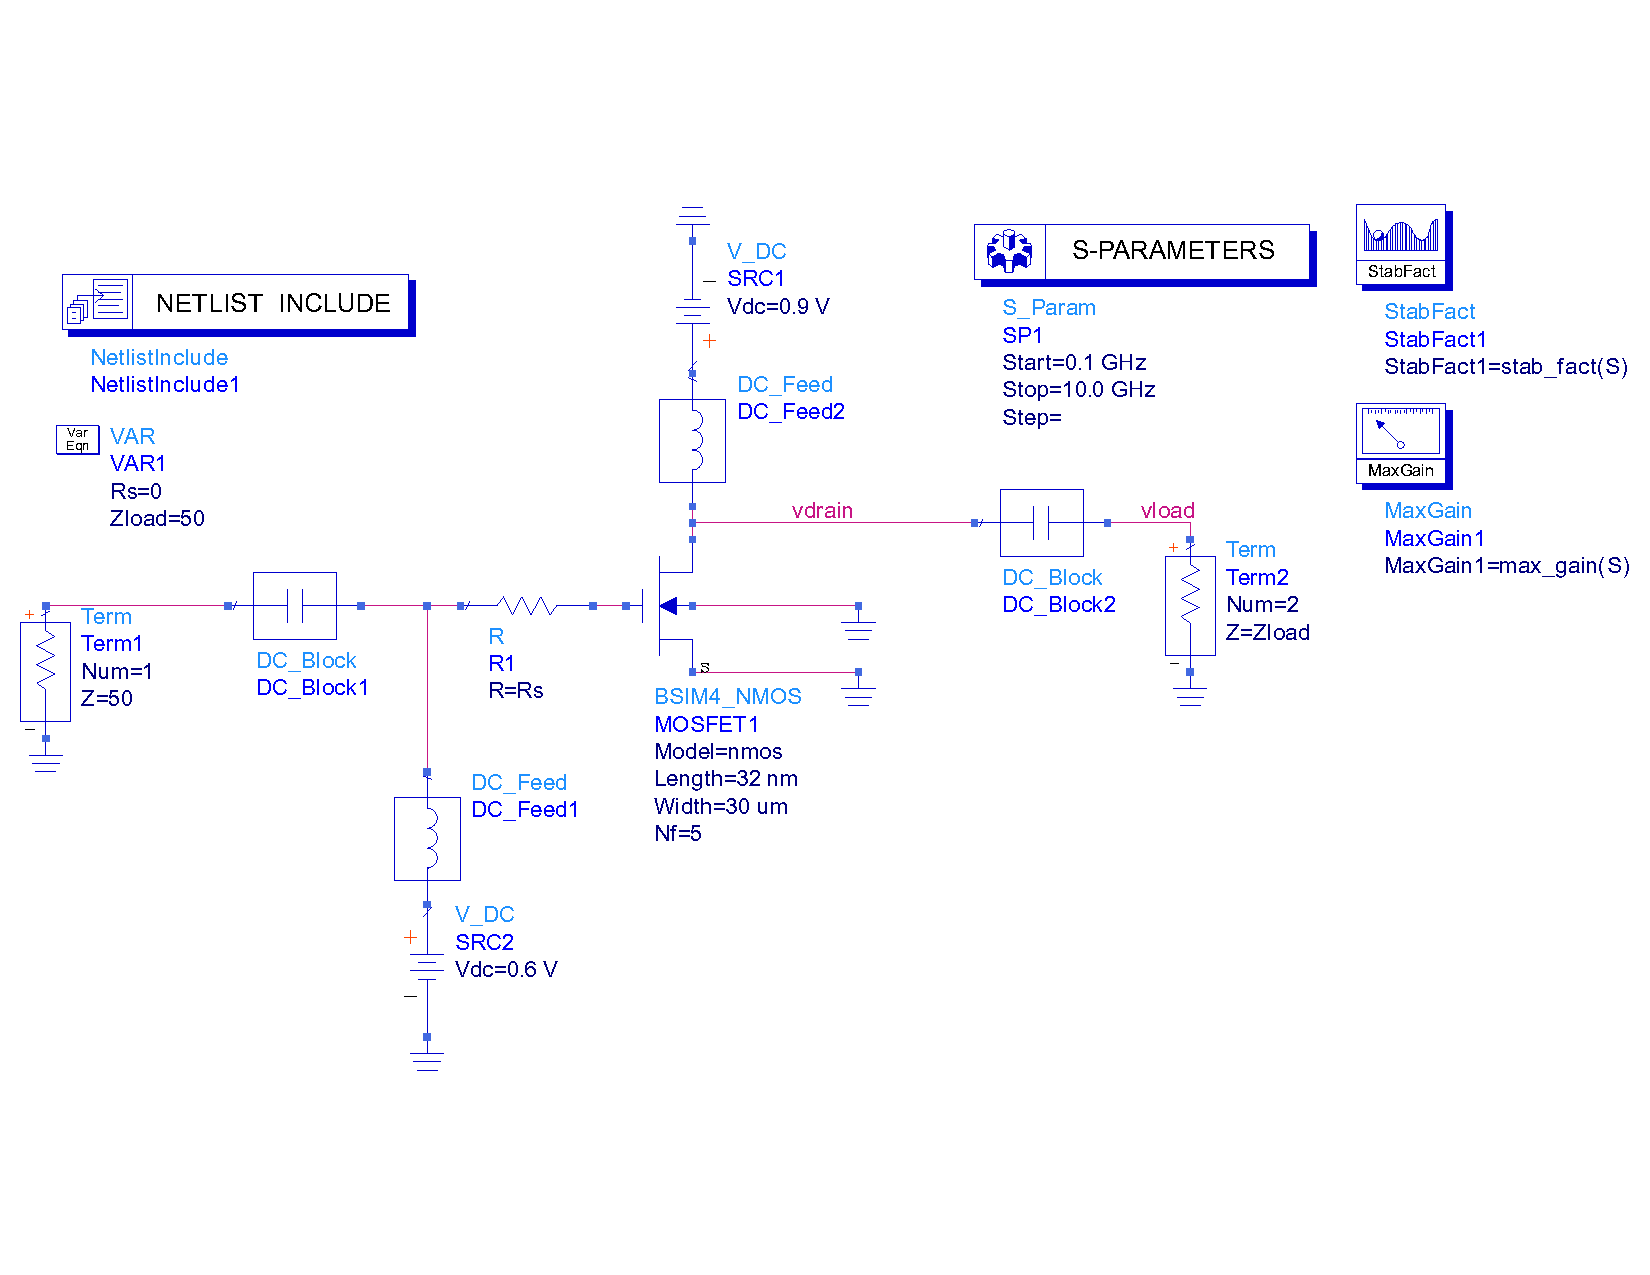
\includegraphics[width=\linewidth]{partb_stability_schematic.pdf}
    \caption{Stability Factor Testbench}
    \endminipage\hfill
    \minipage{0.50\textwidth}
    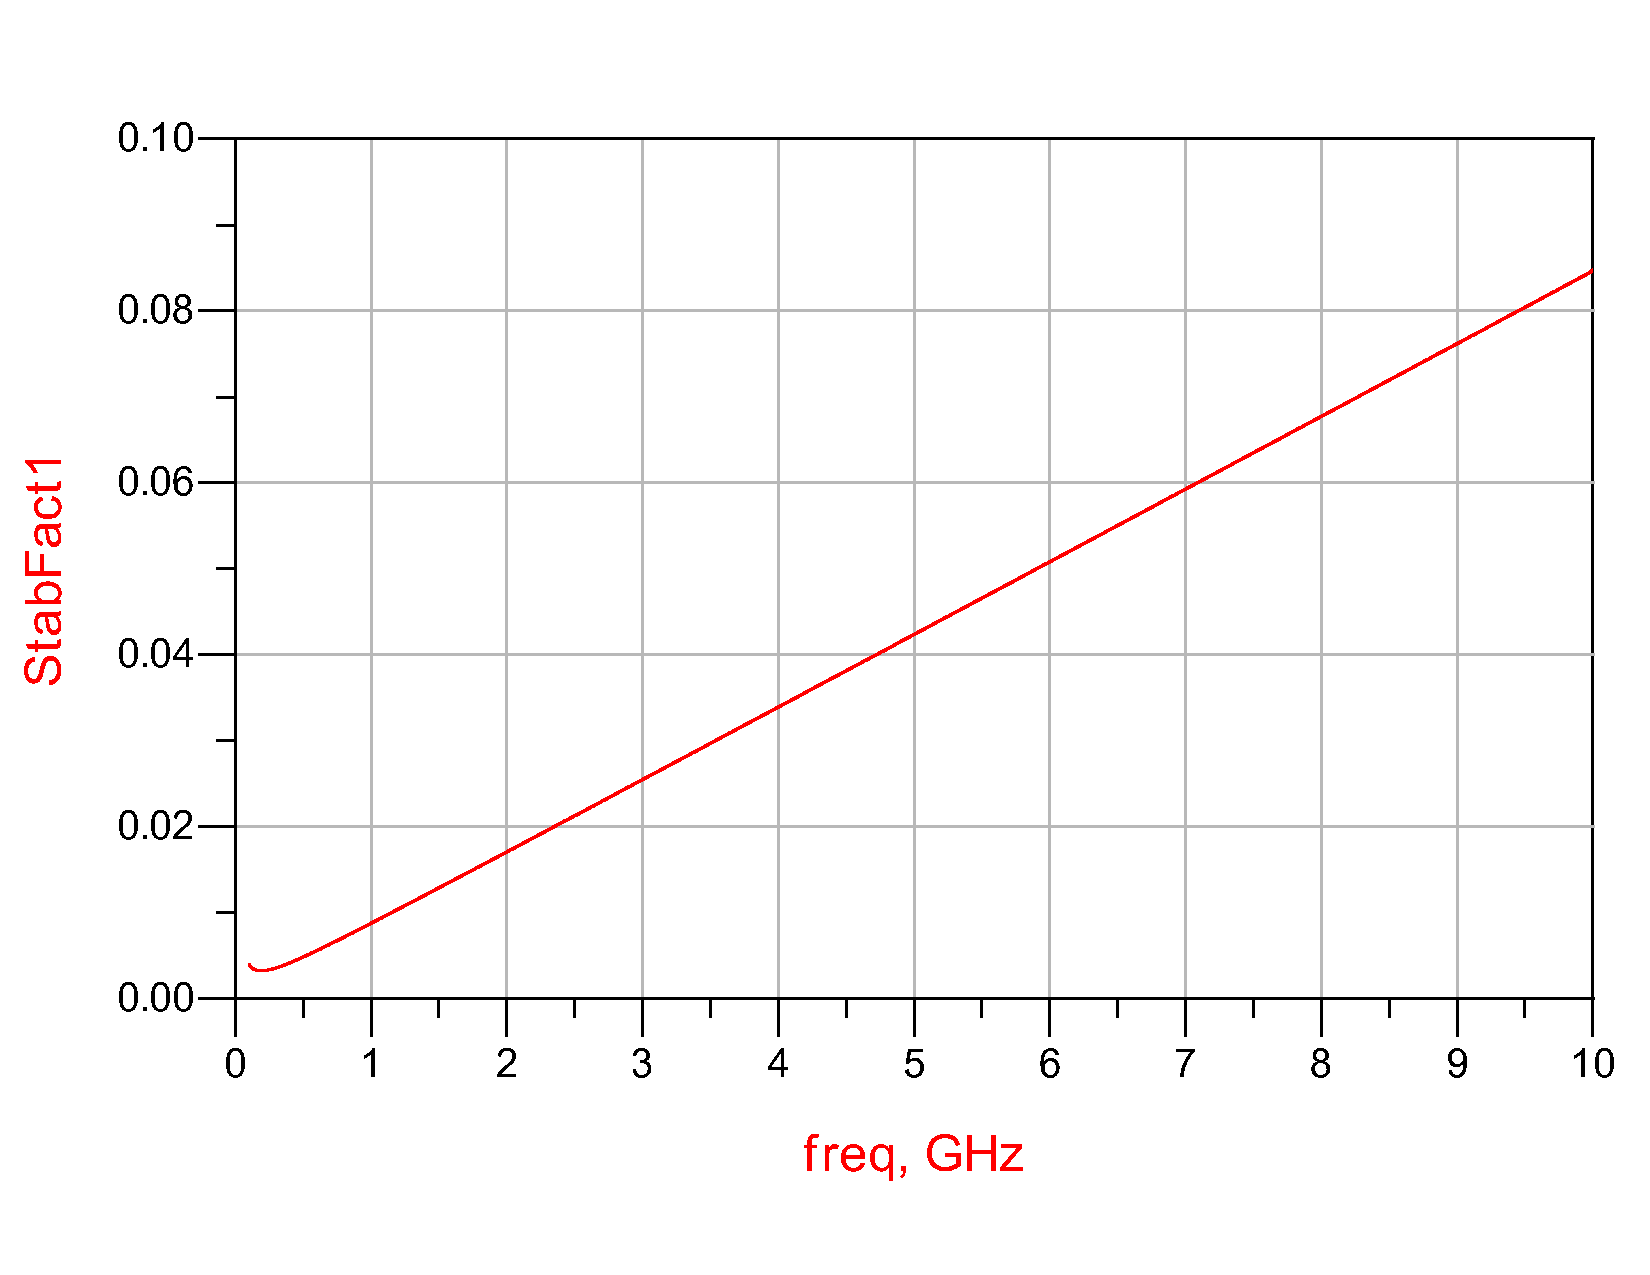
\includegraphics[width=\linewidth]{partb_stability_factor_vs_frequency.pdf}
    \caption{Stability Factor vs. Frequency}
    \endminipage
\end{figure}

The transistor is not unconditionally stable at 1 Ghz. To find a passive load impedance that gives a negative real impedance, we can use the stability analysis (circle) feature of ADS.

\begin{figure}[H]
    \minipage{0.47\textwidth}
    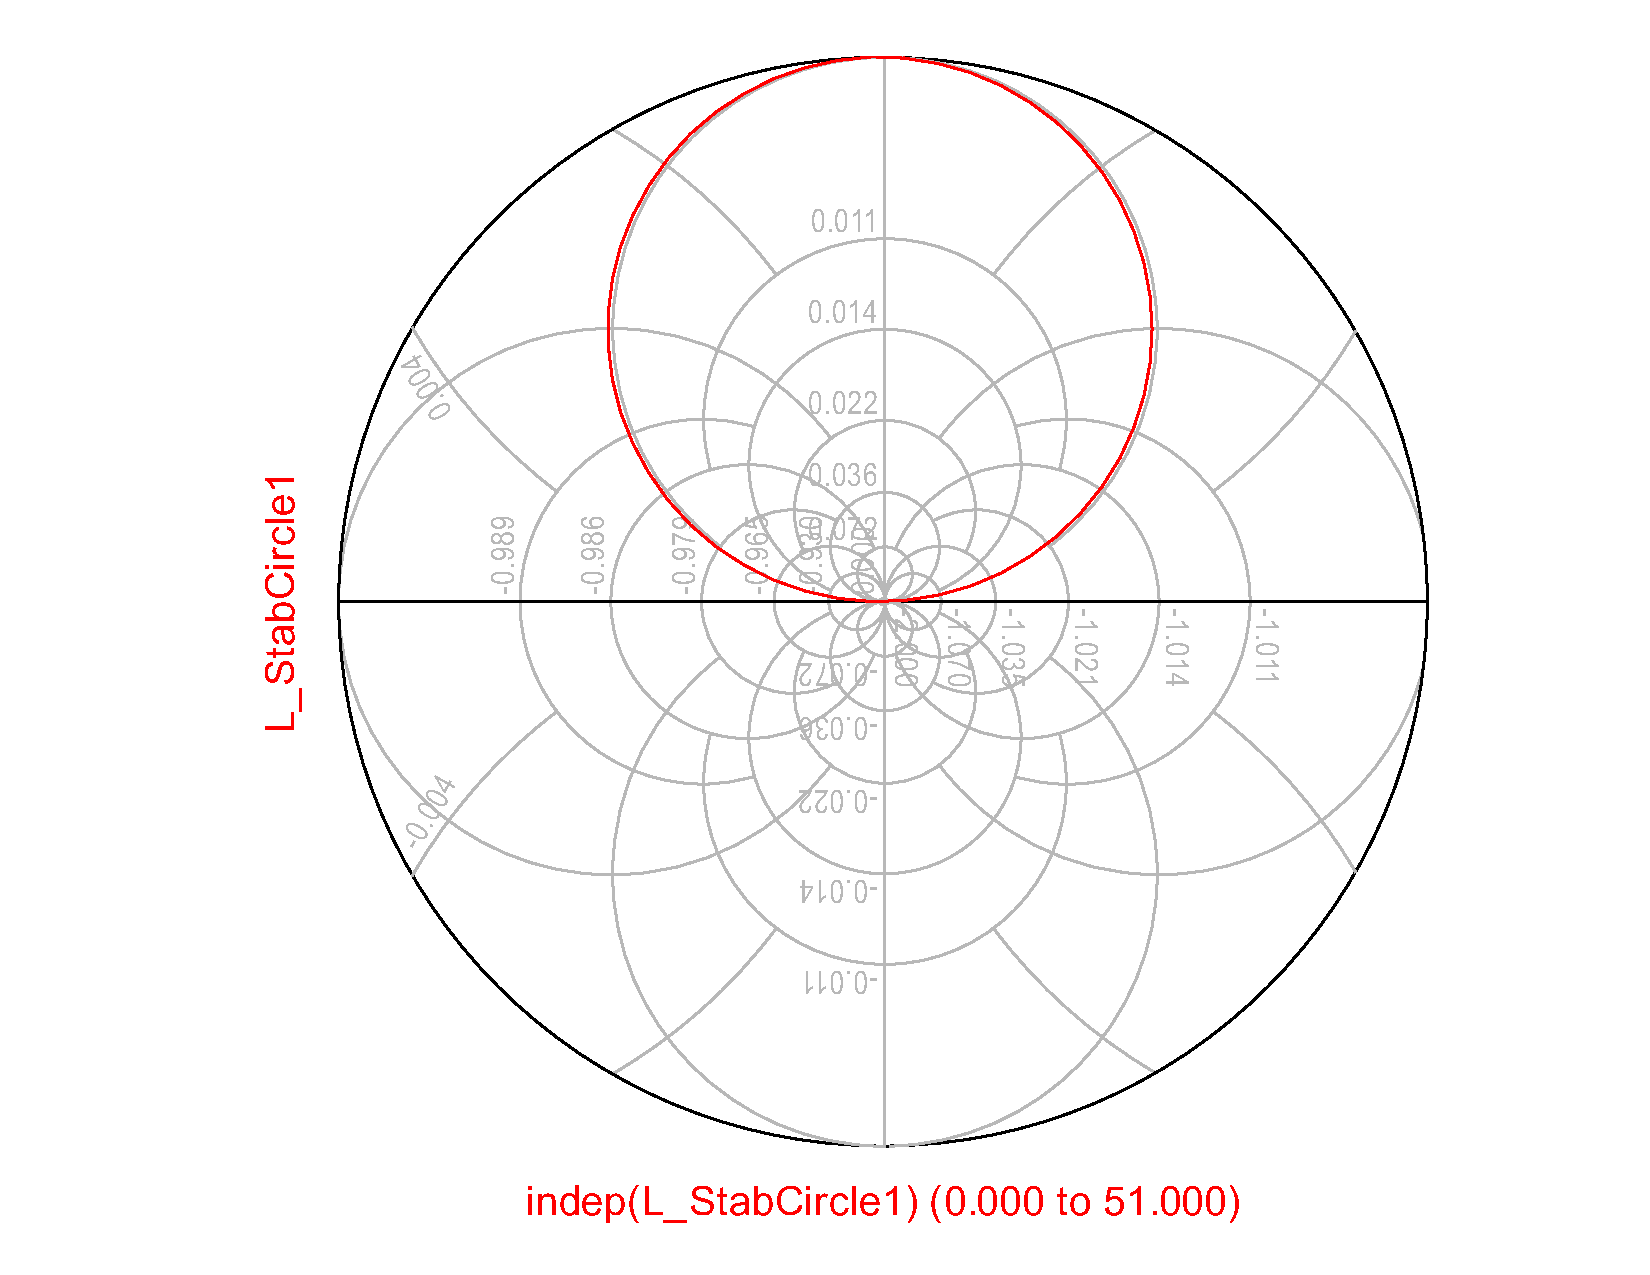
\includegraphics[width=\linewidth]{partb_stability_circle.pdf}
    \caption{Load Stability Circle (not scaled to unit impedance circle)}
    \endminipage\hfill
    \minipage{0.47\textwidth}
    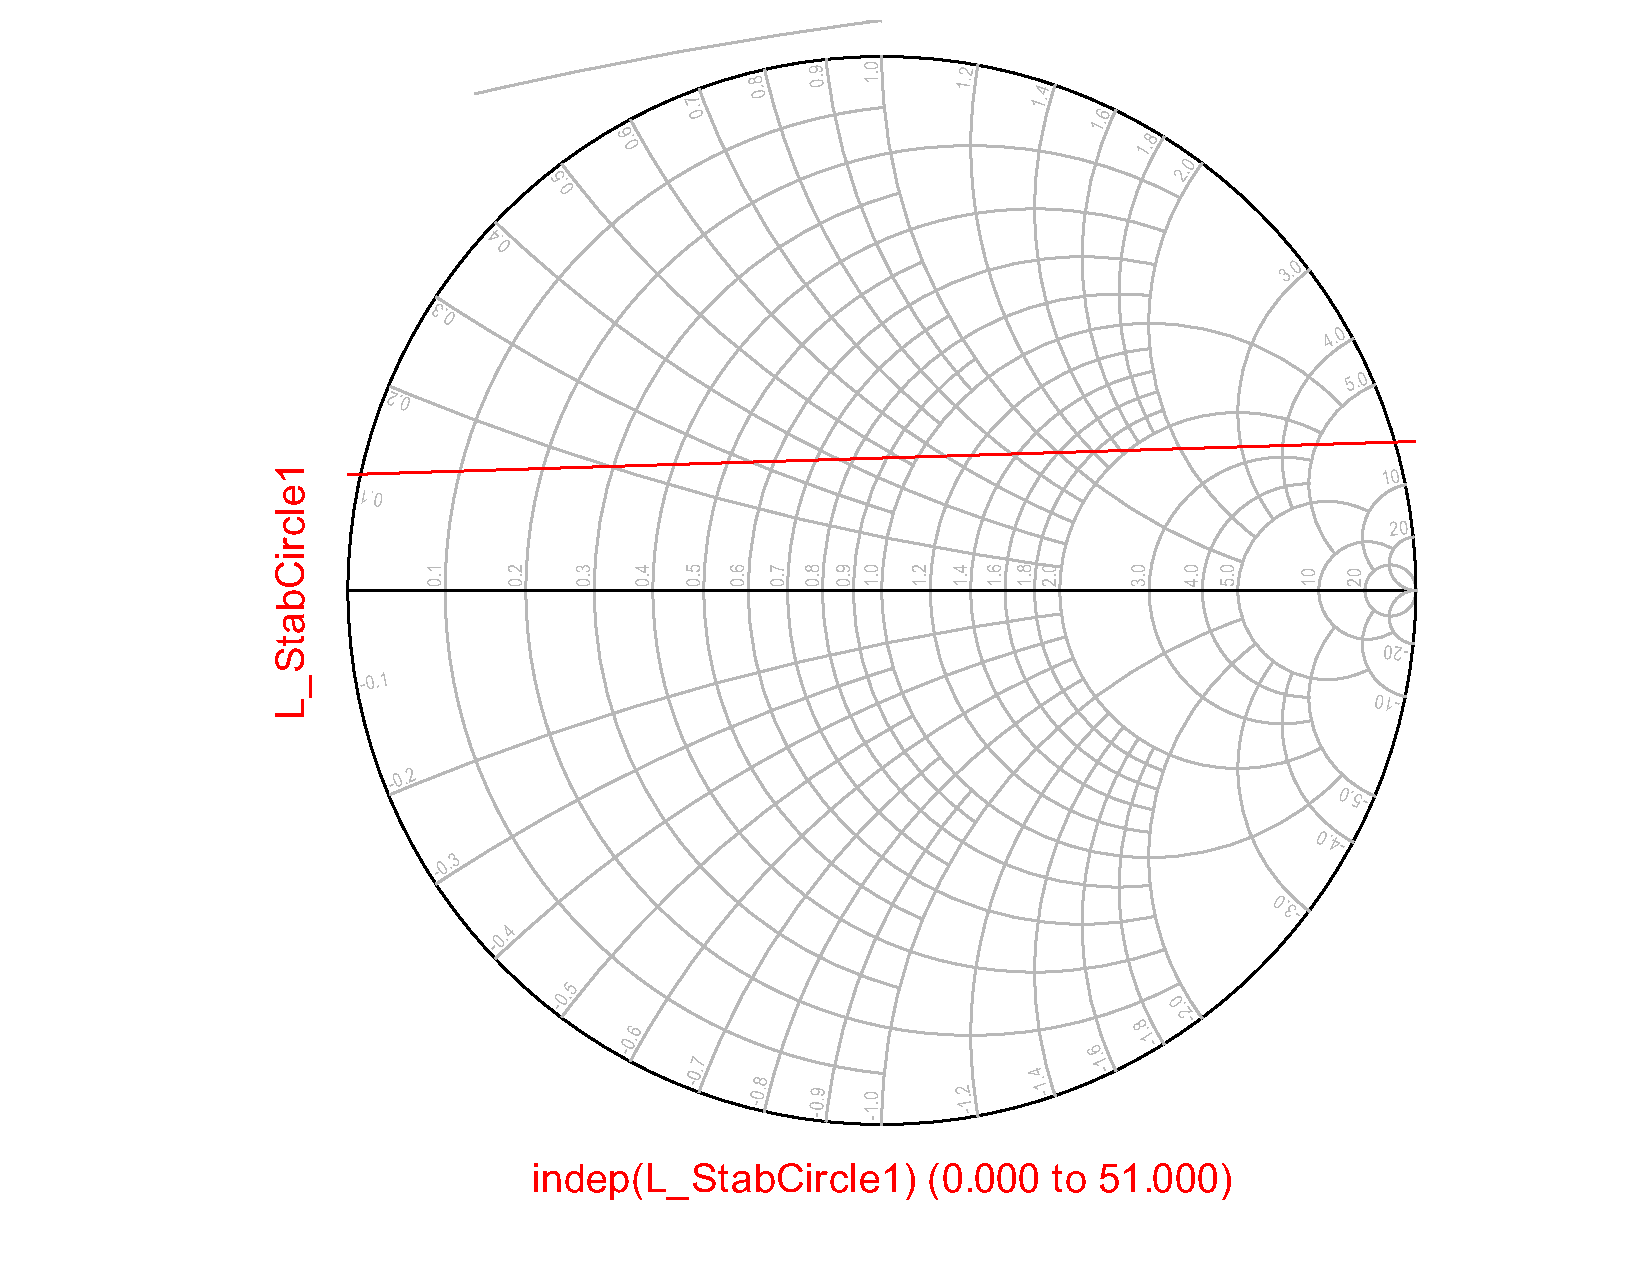
\includegraphics[width=\linewidth]{partb_stability_circle_scaled.pdf}
    \caption{Load Stability Circle (in unit impedance circle)}
    \endminipage
\end{figure}

It can be seen that for sufficiently inductive loads, the transistor isn't stable. For instance a load of $Z_L = 50 + 1.2j$ will lead to a negative input impedance.
\begin{figure}[H]
    \centering 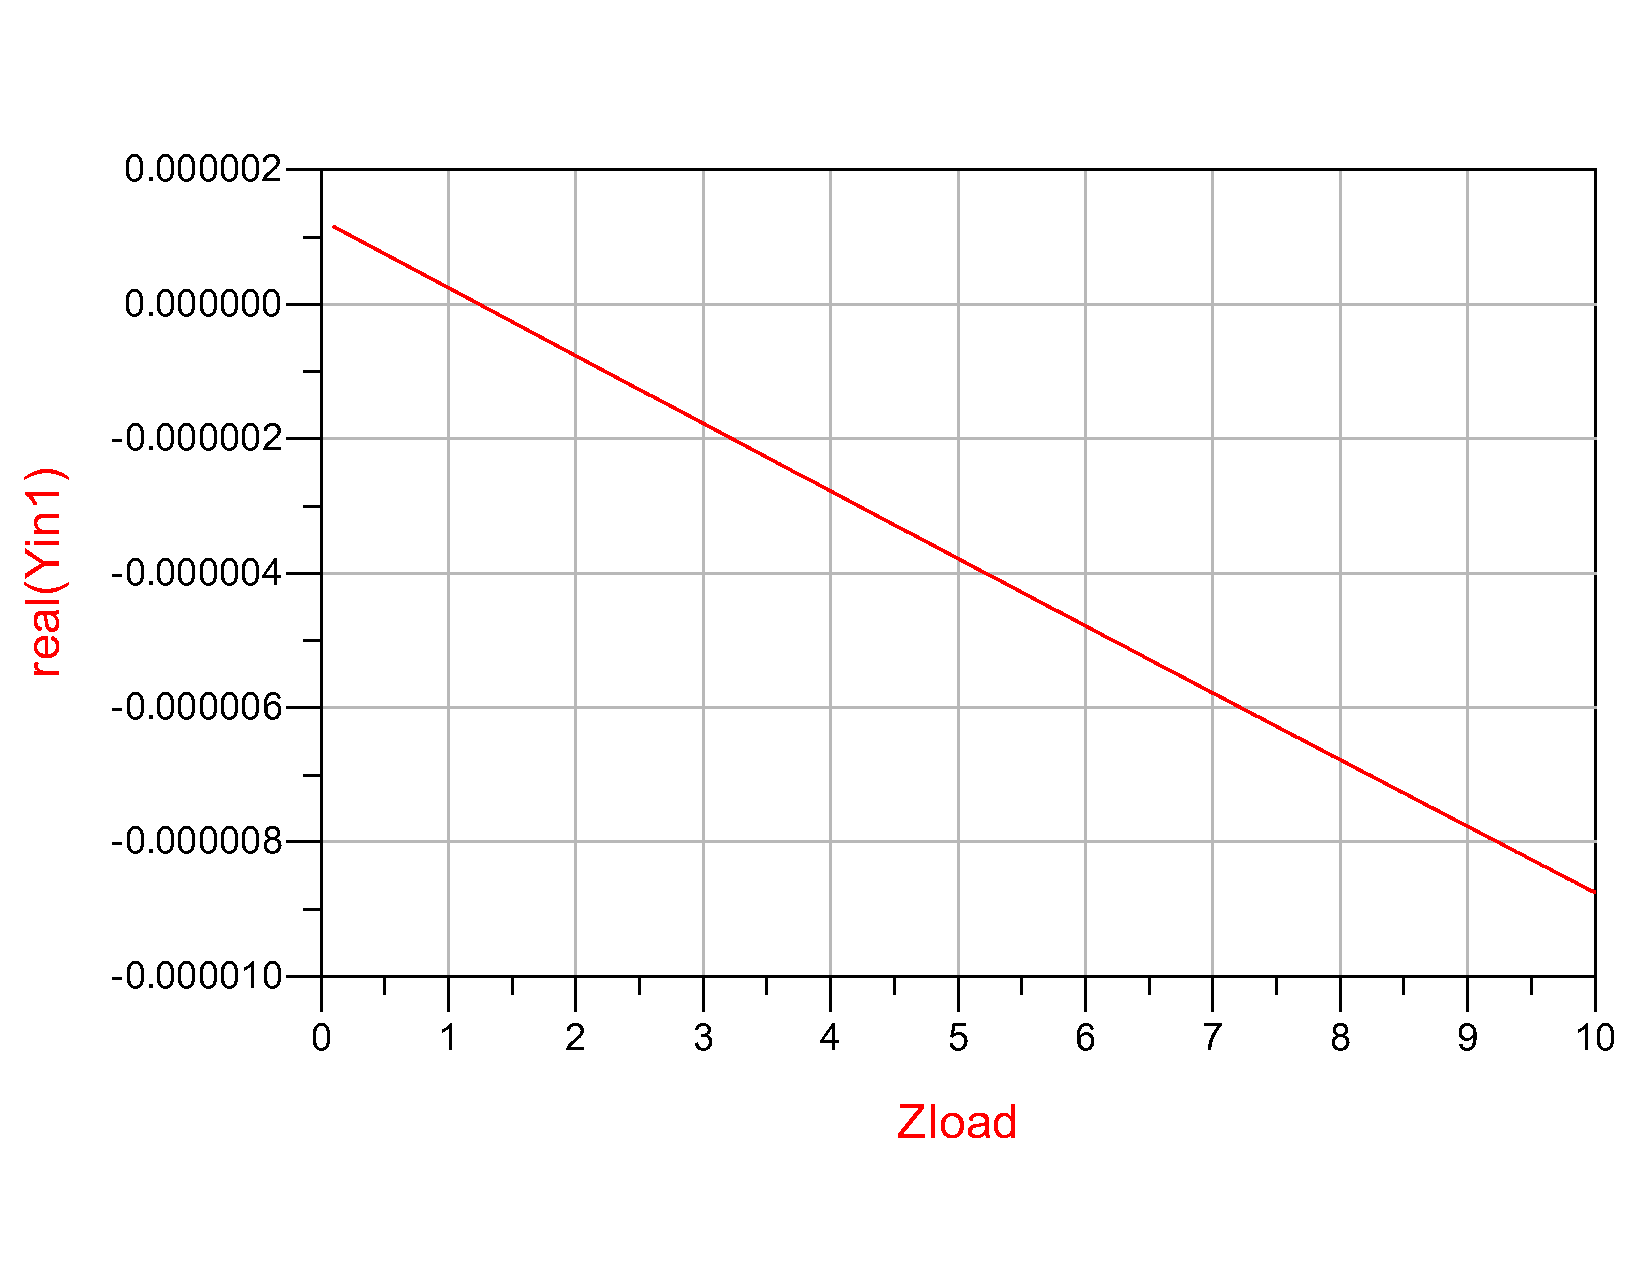
\includegraphics[width=\linewidth-6cm]{partb_yin_vs_zload.pdf}
    \caption{$Z_L = 50 + j Z_{load}$}
\end{figure}

\subsection{Move Pole to Im Axis}
{\color{blue} Following (b), find the passive source impedance at 1 Ghz that moves the system pole to the imaginary axis.}

If the system pole is moved to the imaginary axis, it indicates that the system is marginally stable.
This would correspond to when the system poles for this circuit move from possible instability to certain stability by changing the source impedance.
We can plot the source stability circle and take a point right on the circle.
\begin{figure}[H]
    \centering 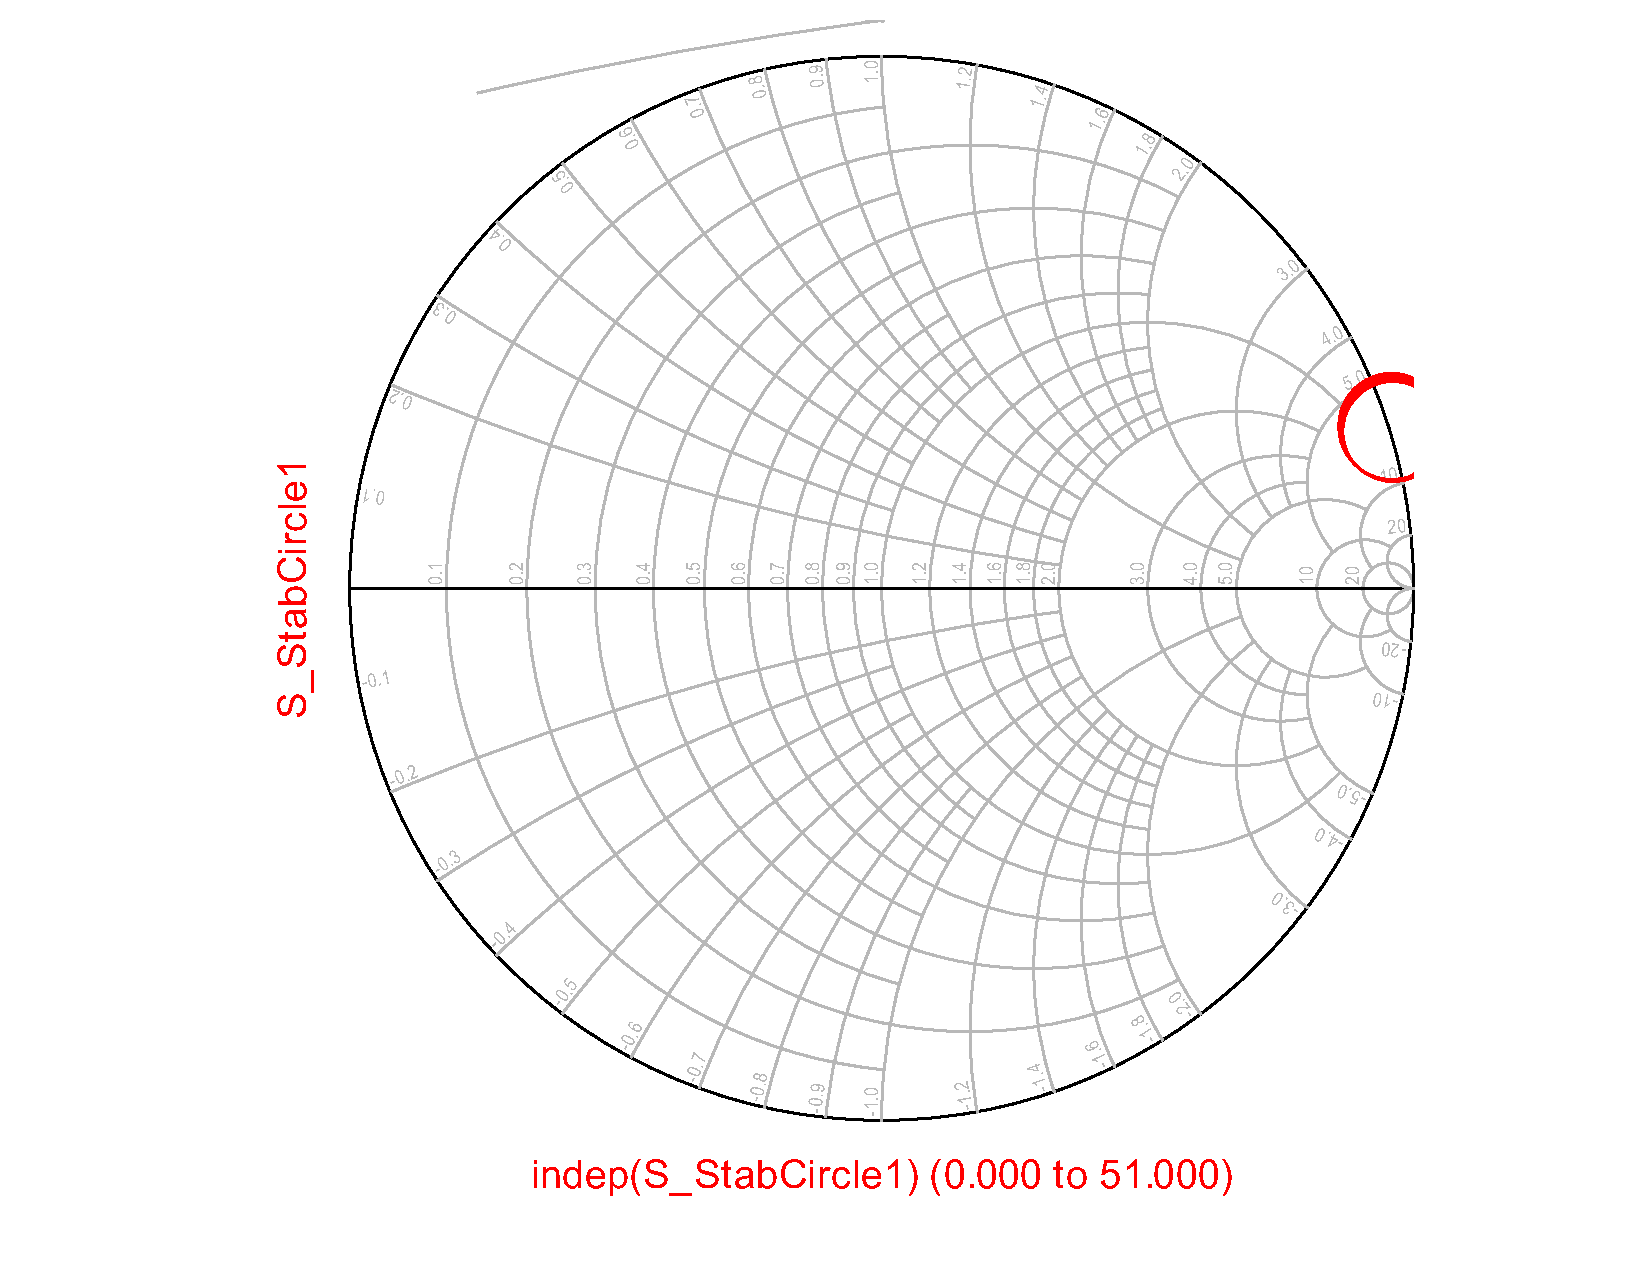
\includegraphics[width=\linewidth-6cm]{partc_stability_circle.pdf}
    \caption{Source Stability Circle}
\end{figure}
We can immediately read off a value of $Z_s = 1.0 + 5j$ (normalized to 50 $\Omega$).

\subsection{Stabilize with Series Resistor}
{\color{blue} Add a series resistor at the transistor gate to make the device unconditionally stable at 5 Ghz with $k=1.2$.
What is the resistor value and the maximum transducer gain of this new device (FET+resistor) at 5 Ghz?
Plot $k$ versus frequency}

\begin{figure}[H]
    \minipage{0.47\textwidth}
    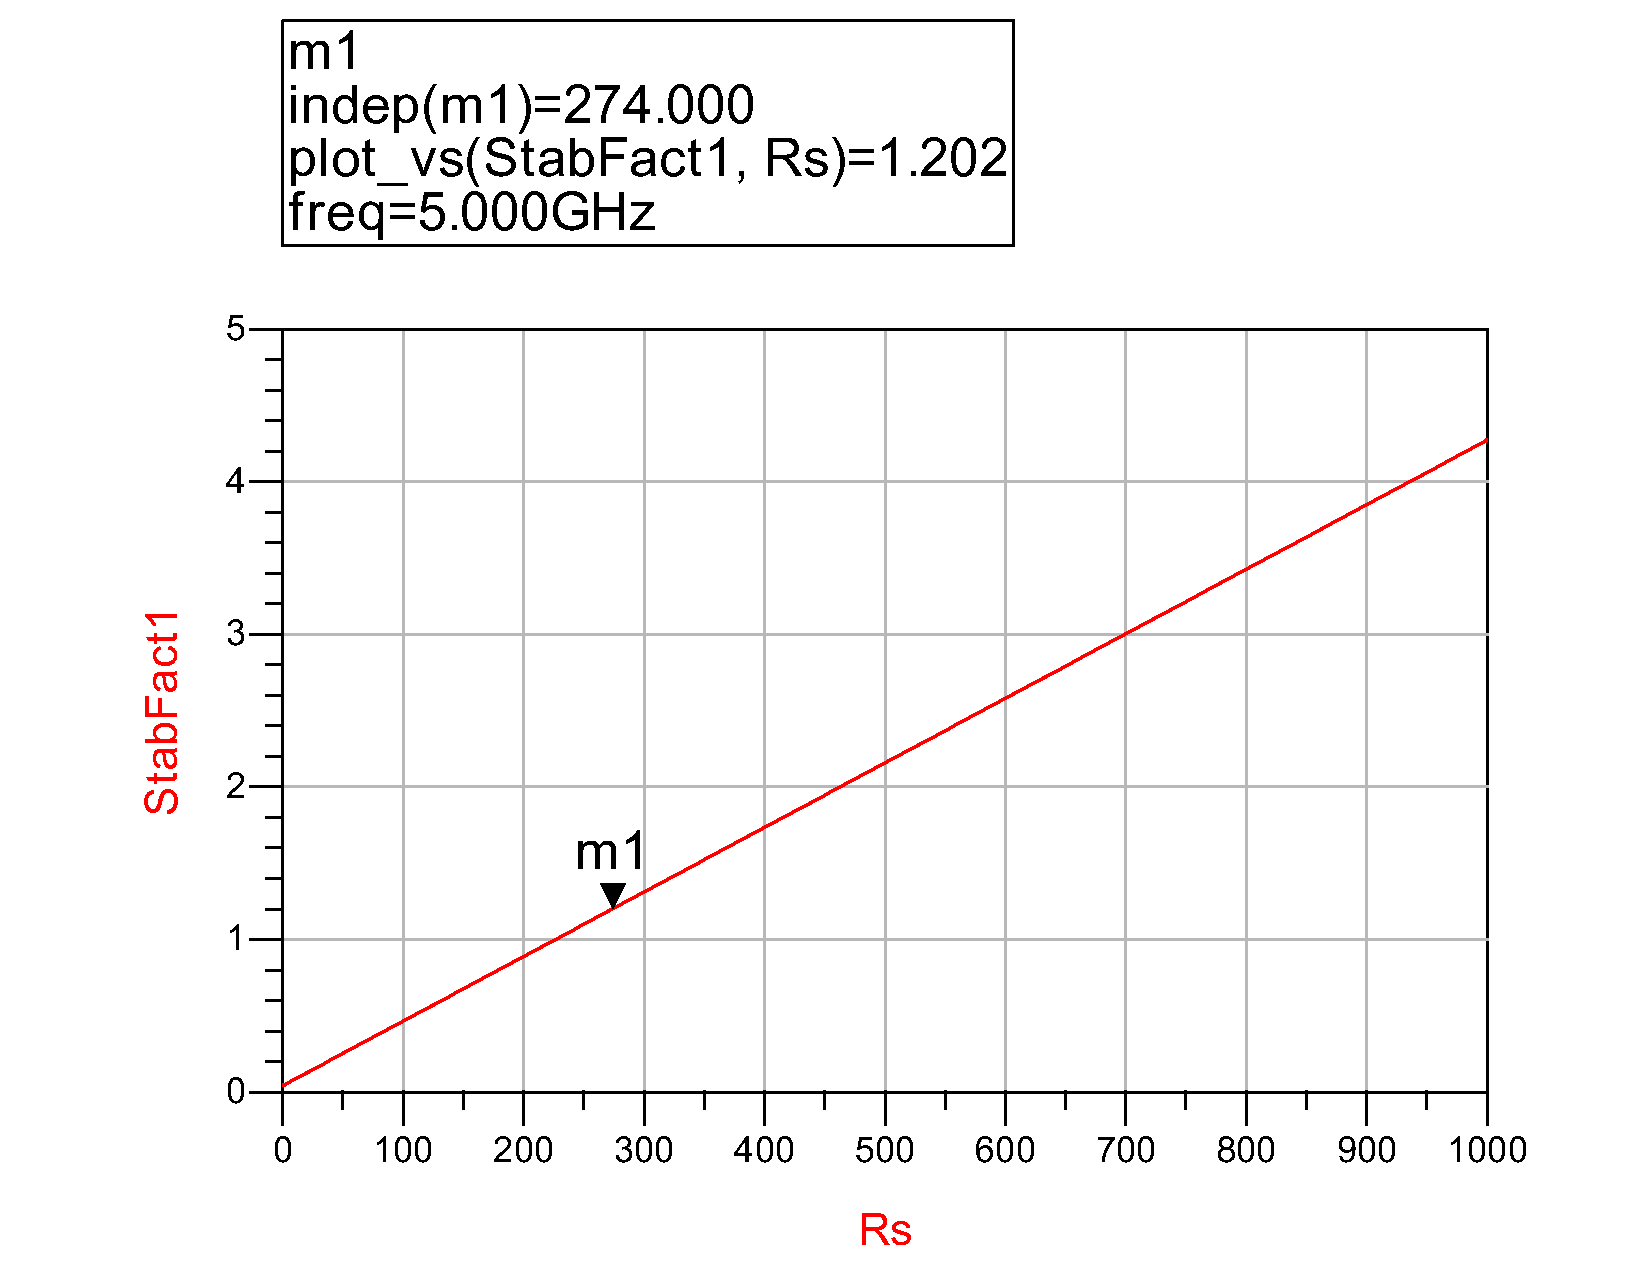
\includegraphics[width=\linewidth]{partd_rs_sweep.pdf}
    \caption{Series resistance sweep vs. K}
    \endminipage\hfill
    \minipage{0.47\textwidth}
    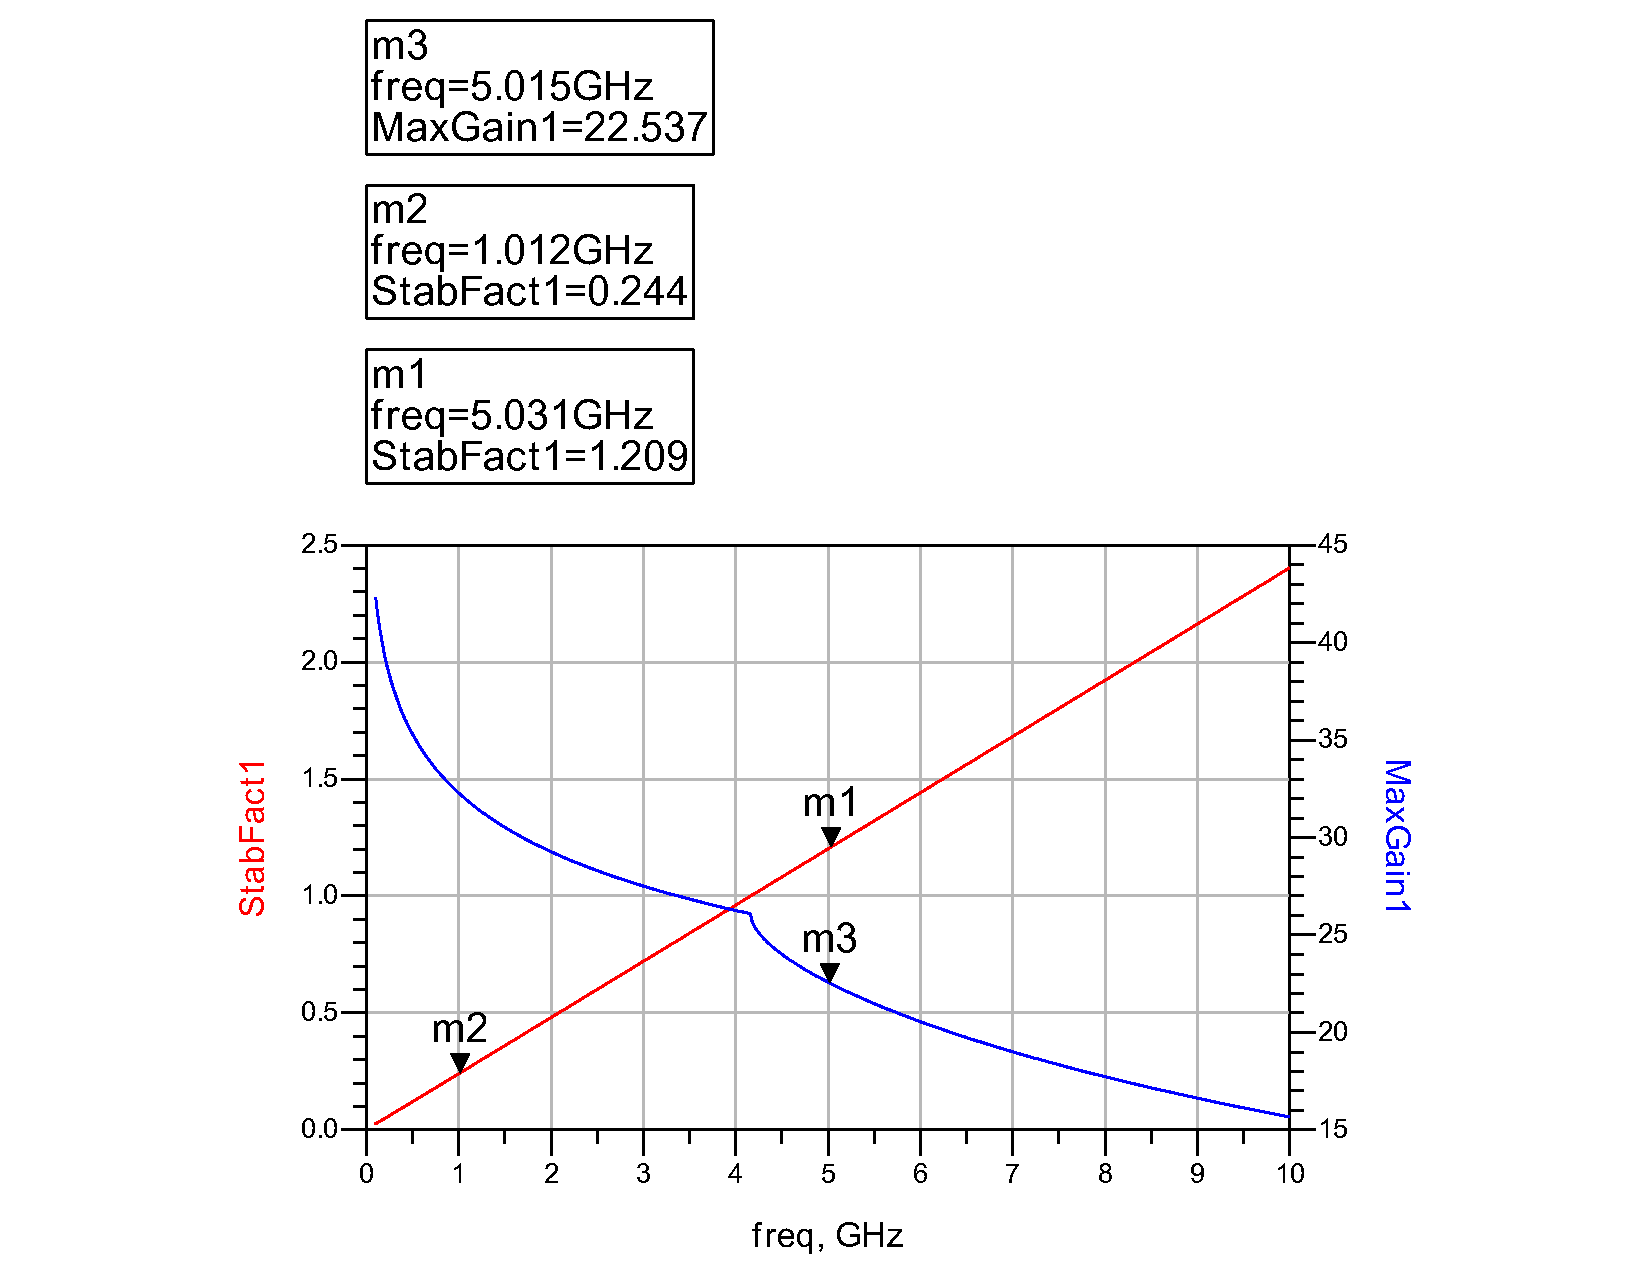
\includegraphics[width=\linewidth]{partd_stability_and_gain_vs_freq.pdf}
    \caption{Stability and Gain of Device at 5 Ghz}
    \endminipage
\end{figure}

We see an ideal series resistance of $274 \Omega$ and a max gain of 22.5 dB.

\subsection{Drawbacks of Series Resistance}
{\color{blue} The new device still has $k < 1$ as 1 Ghz, which is undesireable because the load and source impedances of a 5 Ghz design are usually not controlled at 1 Ghz.
Therefore, a pair of undesired source and load impedances at 1 Ghz can make the system unstable and the 5 Ghz amplifier is no longer useable.
Further increasing the series resistor can make $k > 1$ at 1 Ghz.
What is the main drawback of this approach?}

The main drawback is losing maximum transducer gain. As the source resistance increases, it dissipates more power and the overall power gain of the circuit is reduced.

\subsection{Max Voltage Gain and Power Gain}
{\color{blue} We will eventually make $k > 1$ at all frequencies with a better method. Let's focus on the 5 Ghz design for now. Assuming the source resistor is $50 \Omega$, what is the voltage gain ($V_{in,mixer}/V_s$) and power gain ($P_{in,mixer}/P_{avs}$) without any matching network?}

We use a $50 \Omega$ source resistance and the gate resistance from part (d) to stabilize the amplifier at 5 Ghz. The load is replaced with the mixer input impedance model.

To use a standard S-parameter termination, we use a parallel to series conversion.

\begin{align*}
asdf
\end{align*}


\end{document}
